\section{Diskussion}
\label{sec:Diskussion}

In \autoref{sec:Auswertung} wurde für die Acrylplatte sowohl mit der Schieblehre, als auch mit der Ultraschallmethode eine Dicke von $D = \SI{6}{\milli\meter}$
bestimmt. \newline
Bei der Messung der Periodenlängen wurde ein Wert von $\SI{0,5}{\micro\second}$ theoretisch vorausgesagt, was durch die am Ultraschallgerät eingestellte
Frequenz erfolgte. Mit dem Ultraschallgerät wurde ein Wert von $\SI{0.546 \pm 0.028}{\micro\second}$ gemessen, was einer Abweichung von $(9 \pm 6)$ \%
entspricht. Es ist somit zu sagen, dass die Theorie bestätgt wurde. \newline
Die Schallgeschwindigkeit wurde einmal mit dem Impuls-Echo-Verfahren und einmal mit der Durchschallungsmethode bestimmt. Die Ergebnisse und der Theoriewert \cite{SchallgeschwAcryl} lauten wie folgt,
\begin{align*}
    \nu_{\text{Echo}} &= \SI{1,84 \pm 0,24 e3}{\meter\per\second\squared}, \\
    \nu_{\text{Durchschall}} &= \SI{2.73 \pm 0.04 e3}{\meter\per\second\squared}, \\
    \nu_{\text{Lit}} &= \SI{2750}{\meter\per\second\squared}.
\end{align*}
Die gemessene Schallgeschwindigkeit bei der Impuls-Echo-Methode entspricht einer Abweichung von $(33 \pm 9)$ \%. Bei der Durchschallungsmethode entspricht der
Wert einer Abweichung von $(0,6 \pm 1,5)$ \%. \newline
Der Grund für die hohen Abweichungen bei der Impuls-Echo-Methode kann das verwendete Kontaktmittel sein. In dem Versuch wurde destilliertes Wasser verwendet um der Dämpfung des Ultraschalles
in Luft vorzubeugen. Mit Koppelgel, das sonst in der Ultraschalltechnik verwendet wird, hätten die Messungen eventuell genauer verlaufen können. \newline
Somit kann bei der mit der Impuls-Echo-Methode gemessenen Schallgeschwindigkeit nicht davon gesprochen werden, dass die Theorie verifiziert wurde. Die Abweichung ist zu groß.
Bei der anderen mit der Durchschallungsmethode gemessenen Schallgeschwindigkeit kann bei dieser geringen Abweichung allerdings die Theorie bestätigt werden. \newline
Zwar kann die Dämpfung nicht mit theoretischen Werten verglichen werden, aber es ist bereits an \autoref{fig:plot} zu sehen, dass die Messung nicht genau sein kann.
Es konnten hier nur vier Werte aufgenommen werden, wovon einer signifikante Abweichungen aufwies und somit bei der Auswertung der Dämpfung ausgenommen wurde.
Der Grund, weshalb bei dieser Messreihe nur drei Wertepaare aufgenommen werden konnten ist der, das ein Fehler in der Durchführung unterlaufen ist.
Bei der Durchführung des Versuches wurden mehrere Zylinder aufeinandergestapelt. Allerdings wurde nur der erste Peak gemessen, der einer Reflexion an der Grenzfläche zwischen den beiden
Zylindern entspricht. Anstatt also einen "neuen", längeren Zylinder zu messen, wurde nur der erste Zylinder erneut gemessen. Diese Werte sind demnach für die Auswertung nutzlos. \newline
Die Messreihe des Augapfelmodells kann ebenfalls nicht mit theoretischen Werten verglichen werden, allerdings liegen alle Werte in einer realistischen Größenordnung.


\printbibliography{}

\section*{Anhang}
\label{sec:anhang}

\begin{figure}[H]
    \centering
    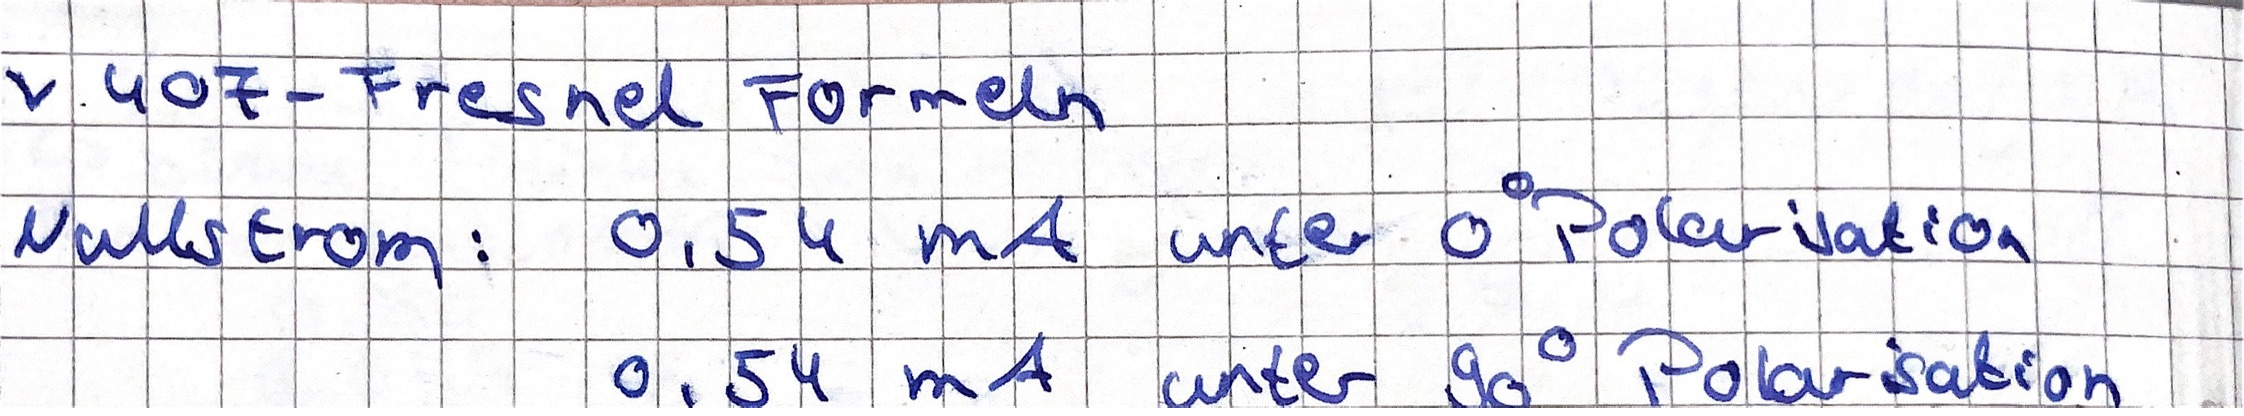
\includegraphics[width=0.7\textwidth]{data/origDaten1.png}
    \caption{Originale Messdaten.}
    \label{fig:origDaten1}
\end{figure}

